\documentclass[conference]{IEEEtran}
\usepackage[utf8]{inputenc}
\usepackage[T1]{fontenc}
\usepackage[spanish,es-noshorthands]{babel}
\usepackage{graphicx}
\usepackage{booktabs}
\usepackage{tabularx}
\usepackage{array}
\usepackage{underscore}
\usepackage{url}
\usepackage{amsmath}
\usepackage{amssymb}
\usepackage{textcomp}
\usepackage{microtype}
\usepackage{caption}
\usepackage[hidelinks]{hyperref}

\captionsetup{font=small}
\newcolumntype{Y}{>{\raggedright\arraybackslash}X}
\renewcommand{\arraystretch}{1.1}

\title{FitTrack: microservicios en Docker Swarm y análisis distribuido con Apache Spark}

\author{
\IEEEauthorblockN{Juan Camilo Serrano, Lucio Matías Melendez Rojas, Juan David Ocampo Gutierrez,\\
Nicolás Castro Pacheco, Diego Fernando Asprilla Palacios}
\IEEEauthorblockA{Curso de Redes e Infraestructura\\
Universidad Autónoma de Occidente\\
Cali, Colombia\\
Noviembre de 2026}
}

\begin{document}
\maketitle

\begin{abstract}
Este trabajo presenta el despliegue de FitTrack, una aplicación de seguimiento físico basada en
microservicios y API REST, sobre un clúster Docker Swarm de dos nodos, y la construcción de un
pipeline de análisis de datos con Apache Spark que alimenta un dashboard. La aplicación se empaquetó
en seis servicios y tres bases de datos, con HAProxy como punto de entrada y balanceo. El pipeline
procesa un dataset sintético de 100.000 usuarios y 8,4 millones de filas, aplica limpieza de
duplicados, fechas y unidades, y calcula KPIs de retención, adherencia, metas y evolución de peso.
Los resultados se publican por una API y se muestran en una pestaña ``Analítica''. Las pruebas de
carga muestran una mejora de 1,89$\times$ en RPS al pasar de una a tres réplicas, y la validación
contra los patrones sembrados confirma que el análisis recupera las señales del dataset. En la prueba
de failover, matar una de tres réplicas mantuvo el servicio en 99,70\,\% de éxito y recuperó la tarea
en 8 segundos. El trabajo documenta las decisiones, los problemas encontrados y una guía reproducible.
\end{abstract}

\begin{IEEEkeywords}
Docker Swarm, microservicios, Apache Spark, análisis distribuido, HAProxy, dashboard,
reproducibilidad.
\end{IEEEkeywords}

\section{Introducción}
El módulo de Redes e Infraestructura cubre el empaquetado de aplicaciones, el despliegue en clústeres
de contenedores y el procesamiento de datos a gran escala. El proyecto final integra esas tres
dimensiones sobre una aplicación real: FitTrack, una aplicación de seguimiento físico con servicios
de usuarios, medidas, progreso, rutinas y metas.

El objetivo general es desplegar la aplicación en un clúster de contenedores con escalabilidad y
balanceo, y construir un pipeline de análisis distribuido que genere reportes consumidos por el
dashboard. Los objetivos específicos son: (1) empaquetar los microservicios y sus bases de datos en
imágenes reproducibles; (2) desplegar el stack en Docker Swarm \cite{docker} con HAProxy; (3)
diseñar y ejecutar un ETL con Spark \cite{spark} sobre un dataset de gran escala; (4) calcular KPIs de
interés y validarlos contra patrones conocidos; (5) publicar los resultados por una API y mostrarlos
en el dashboard; y (6) medir funcionamiento, escalabilidad y desempeño, documentando la reproducción.

La contribución principal es una solución completa y reproducible que separa la aplicación
transaccional (microservicios y bases de datos) del procesamiento analítico (Spark y archivos
Parquet/JSON), con evidencia de funcionamiento y de escalado. El documento sigue el formato IEEE de
dos columnas \cite{ieee}.

\section{Análisis}
\subsection{Dataset}
Se usó \textbf{FitTrack-Synth} \cite{dataset}, un dataset sintético y reproducible generado por el
propio equipo.
El profesor autorizó explícitamente su uso. La decisión se justifica por privacidad (no contiene
datos de personas reales), reproducibilidad (con la semilla 42 se obtiene el mismo dataset) y
validación (el generador siembra patrones conocidos y publica una carpeta \texttt{clave\_respuestas}
para comprobar que el análisis los recupera).

El dataset tiene 100.000 usuarios y 8.462.080 filas crudas (741 MB) en cuatro CSV: usuarios, medidas,
metas y rutinas. Cubre 78 semanas, del 2025-01-06 al 2026-07-05. Incluye suciedad controlada:
duplicados exactos, nulos en medidas, fechas en \texttt{dd/mm/aaaa}, pesos en libras y pesos
absurdos. El validador del generador ejecutó \textbf{24 chequeos OK, 0 con falla}.

La limitación principal es que los datos son sintéticos: los resultados no describen una población
real, pero sí permiten evaluar el pipeline, la limpieza y la capacidad de recuperar patrones.

\subsection{Alternativas evaluadas}
Se compararon las opciones disponibles para cada dimensión del despliegue; el
Cuadro~\ref{tab:alternativas} resume la decisión y el motivo. El criterio fue doble: usar lo que ya
estaba disponible en el laboratorio y caber en 3,8 GiB de RAM por nodo, porque el objetivo del curso
es demostrar el funcionamiento, no maximizar la sofisticación de las herramientas.

\begin{table}[t]
\centering
\caption{Alternativas evaluadas y decisión.}
\label{tab:alternativas}
\small
\begin{tabularx}{\columnwidth}{@{}l Y@{}}
\toprule
Dimensión & Decisión y motivo \\
\midrule
Orquestación & \textbf{Swarm}: ya estaba inicializado, es nativo de Docker y suficiente para dos
nodos. Kubernetes habría exigido más recursos y complejidad. \\
Balanceo & \textbf{HAProxy}: \texttt{server-template} descubre tareas por DNS y permite
round-robin con health checks. \\
Procesamiento & \textbf{Spark}: escalable, tolerante a fallos y disponible en el laboratorio.
Pandas no cabe cómodamente en 3,8 GiB para 8,4 M de filas; Flink está orientado a streaming. \\
Almacenamiento & \textbf{Parquet + JSON}: separa el batch de la app, evita un esquema nuevo y
permite que el dashboard funcione sin Spark encendido. \\
Visualización & \textbf{Tablas y barras CSS}: sin dependencias externas, funciona offline y se
integra con el frontend existente. \\
\bottomrule
\end{tabularx}
\end{table}

\subsection{Requisitos}
Los requisitos se derivaron del enunciado: despliegue en clúster, escalabilidad, balanceo, pruebas
de desempeño, dataset de gran escala, pipeline de análisis, reportes y dashboard. Se añadieron dos
requisitos no funcionales: reproducibilidad (scripts y README) y operación con recursos limitados
(dos VMs, 3,8 GiB en el servidor).

\section{Diseño}
\subsection{Arquitectura de componentes}
\begin{figure}[t]
\centering
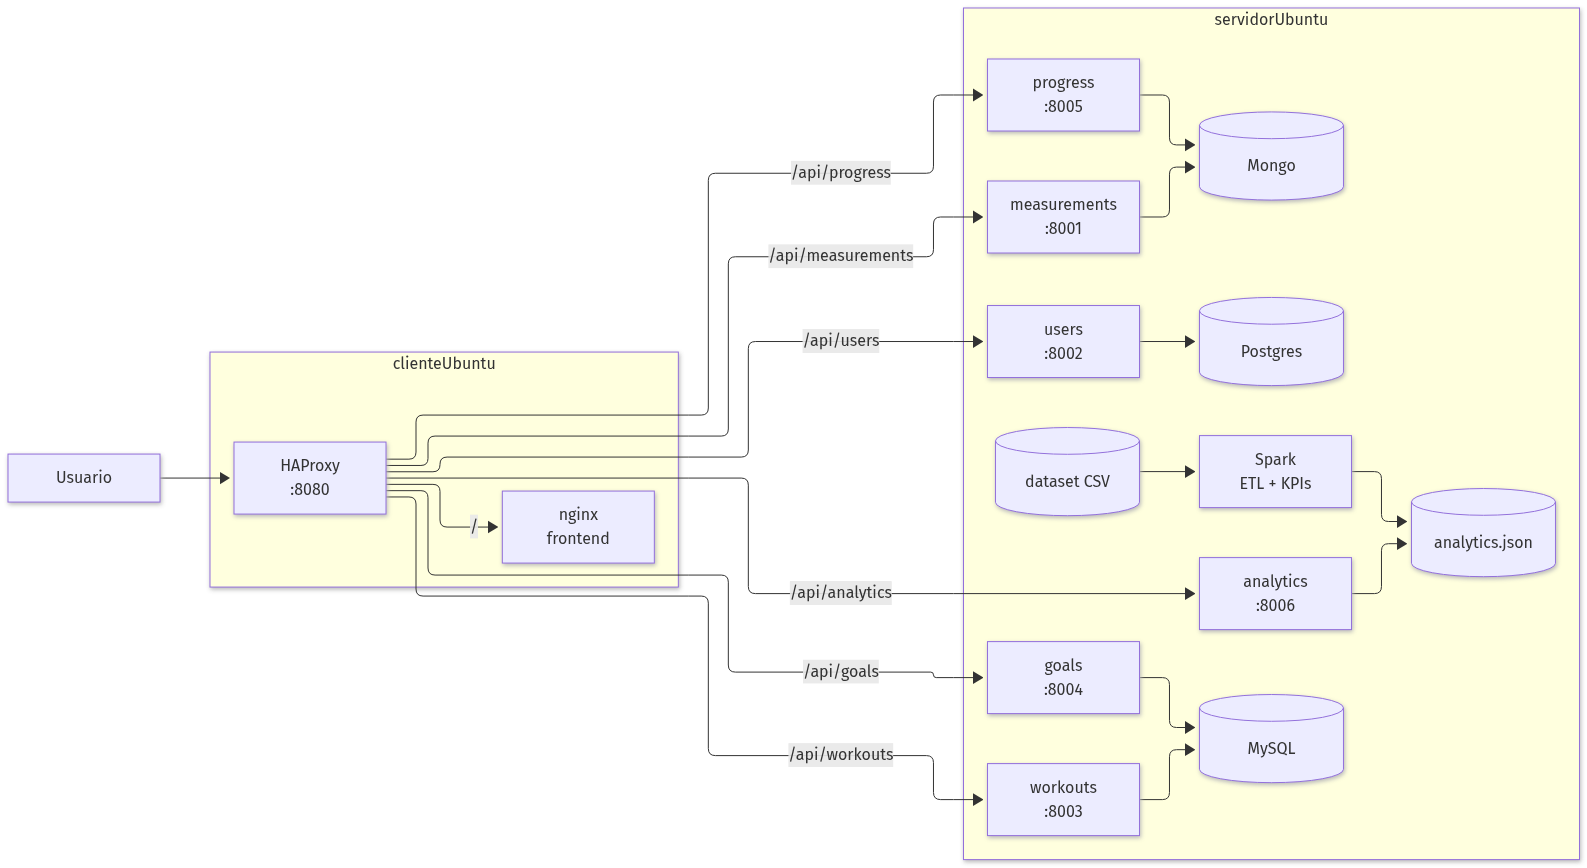
\includegraphics[width=\columnwidth]{figuras/arquitectura.png}
\caption{Componentes y flujo de una petición.}
\label{fig:arquitectura}
\end{figure}

La Figura~\ref{fig:arquitectura} muestra los componentes y el recorrido de una petición. La
aplicación se compone de: \textbf{frontend nginx}, que sirve el HTML/JS del dashboard y no proxea
APIs; \textbf{HAProxy} \cite{haproxy}, único entrypoint que enruta \texttt{/api/<servicio>/} y
balancea entre réplicas; \textbf{users} (registro, login JWT y perfil; Postgres);
\textbf{measurements} (medidas corporales; Mongo); \textbf{progress} (cálculo de progreso; Mongo);
\textbf{workouts} (rutinas; MySQL); \textbf{goals} (metas; MySQL); \textbf{analytics} (API de solo
lectura de los KPIs, en FastAPI \cite{fastapi}); y las bases \textbf{postgres}, \textbf{mongo} y
\textbf{mysql}, con volúmenes \texttt{fittrack\_*}.

El navegador llama a \url{http://192.168.100.2:8080/api/...}; HAProxy reescribe el prefijo y envía
la petición al servicio correspondiente. Los servicios validan el JWT contra \texttt{users} y filtran
por \texttt{user\_id}. La pestaña de analítica llama a \texttt{/api/analytics/dashboard}.

\subsection{Diagrama de despliegue}
\begin{figure}[t]
\centering
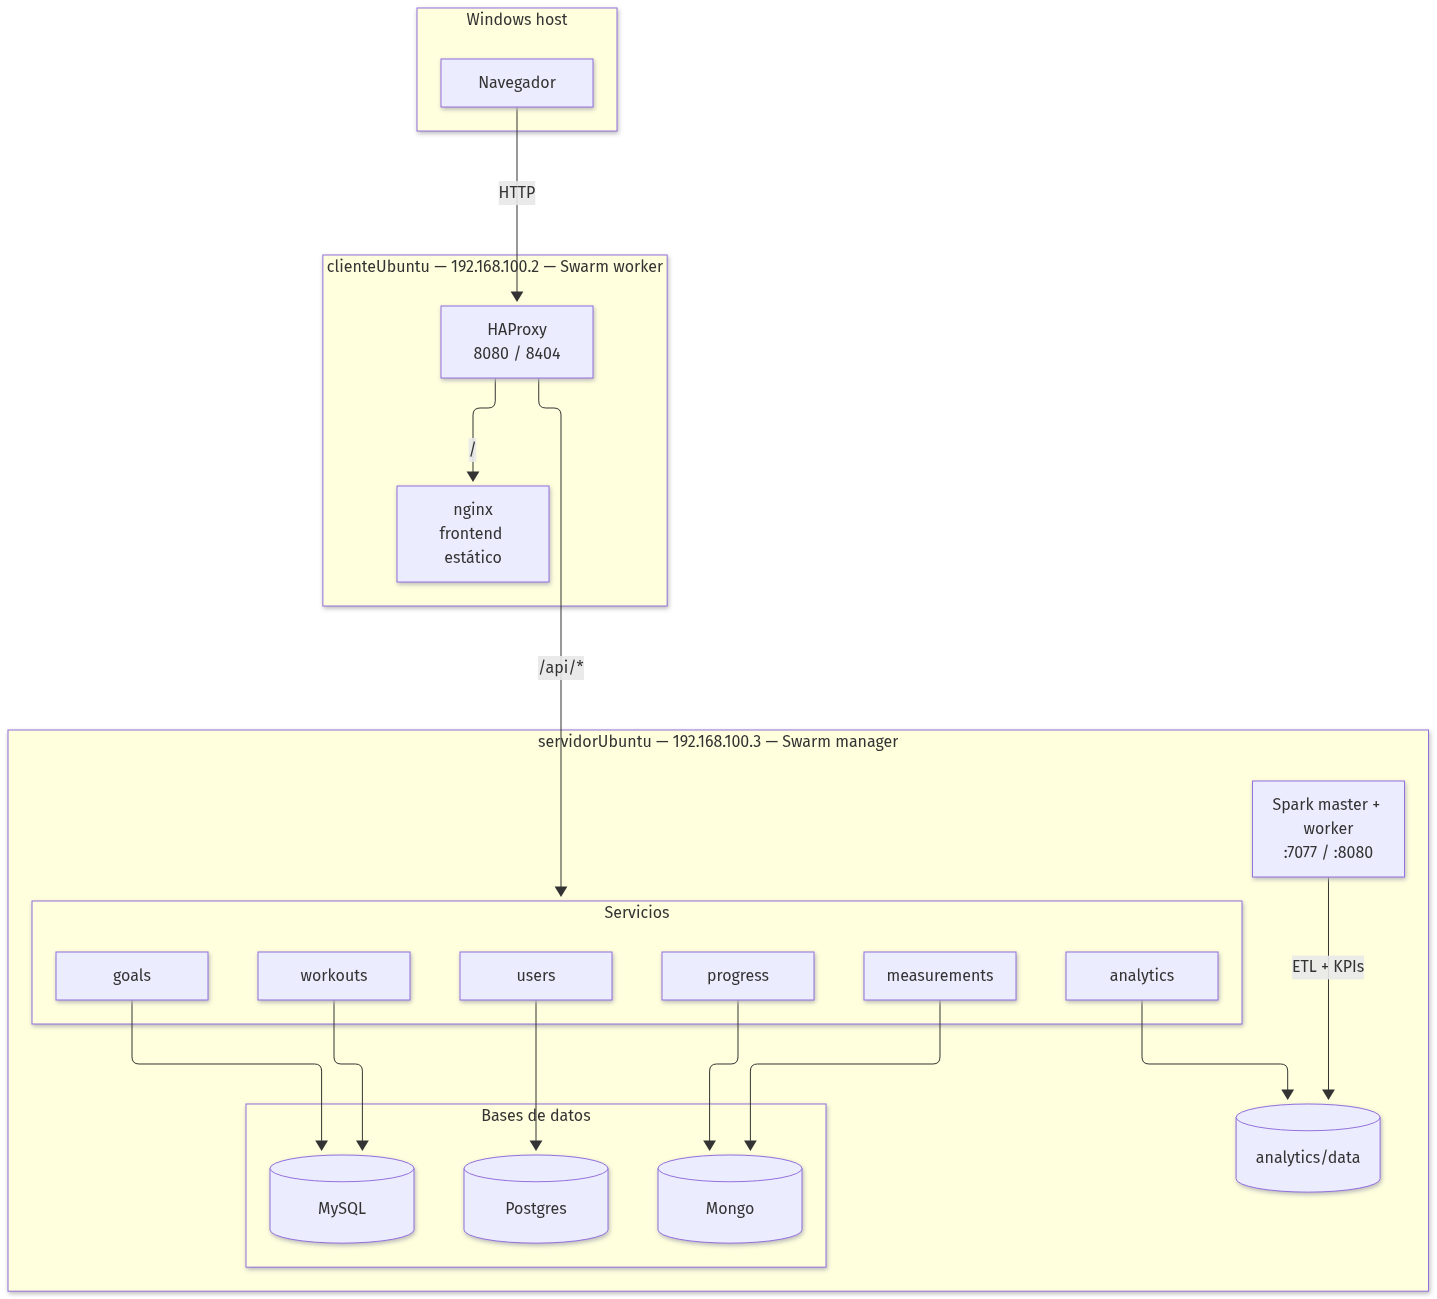
\includegraphics[width=\columnwidth]{figuras/despliegue.png}
\caption{Despliegue en dos VMs y un clúster Spark.}
\label{fig:despliegue}
\end{figure}

\begin{table}[t]
\centering
\caption{Nodos del laboratorio.}
\label{tab:nodos}
\small
\begin{tabularx}{\columnwidth}{@{}l l Y@{}}
\toprule
Nodo & IP & Rol \\
\midrule
\texttt{servidorUbuntu} & 192.168.100.3 & Swarm manager; microservicios, bases de datos,
\texttt{analytics}, Spark master/worker \\
\texttt{clienteUbuntu} & 192.168.100.2 & Swarm worker; nginx y HAProxy \\
\bottomrule
\end{tabularx}
\end{table}

La Figura~\ref{fig:despliegue} y el Cuadro~\ref{tab:nodos} resumen el despliegue. HAProxy y nginx se
fijan al cliente; los servicios con estado y las bases de datos se fijan al servidor para que los
volúmenes y bind mounts estén disponibles. La red overlay de Swarm conecta los dos nodos.

\subsection{Pipeline de datos}
\begin{figure}[t]
\centering
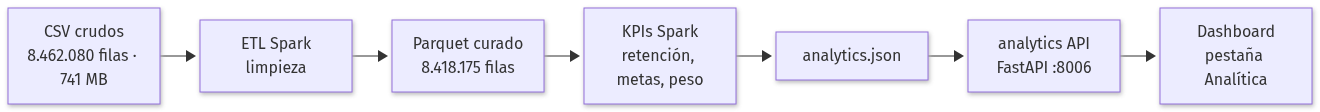
\includegraphics[width=\columnwidth]{figuras/pipeline.png}
\caption{Flujo del dataset al dashboard.}
\label{fig:pipeline}
\end{figure}

La Figura~\ref{fig:pipeline} resume el recorrido. El flujo es: (1) landing zone con los CSV crudos en
\texttt{/root/fittrack/dataset/data}; (2) ETL con esquema explícito, limpieza y escritura de Parquet
en \texttt{analytics/curated}; (3) KPIs con Spark SQL/DataFrame \cite{spark} y escritura de
\texttt{analytics.json}; (4) publicación por el servicio \texttt{analytics}; y (5) consumo por la
pestaña ``Analítica''.

\subsection{Reglas de limpieza}
El ETL aplica un conjunto fijo de reglas, resumido en el Cuadro~\ref{tab:limpieza-reglas}. Cada una
responde a una suciedad sembrada a propósito en el dataset: identificadores repetidos, fechas en dos
formatos, pesos en libras, valores imposibles y metas expresadas en unidades distintas. Solo se
descartan filas en dos casos, duplicados y pesos fuera de rango; los nulos se conservan y las
agregaciones los ignoran.

\begin{table}[t]
\centering
\caption{Reglas de limpieza aplicadas en el ETL.}
\label{tab:limpieza-reglas}
\small
\begin{tabularx}{\columnwidth}{@{}l Y@{}}
\toprule
Problema & Regla \\
\midrule
Duplicados & Eliminar por \texttt{medida\_id} y \texttt{rutina\_id}. \\
Fechas & Aceptar ISO y \texttt{dd/mm/aaaa} con \texttt{try\_to\_date}. \\
Unidades & Convertir peso a kg con \texttt{unidad\_peso}. \\
Pesos absurdos & Descartar fuera de 30--250 kg. \\
Nulos & Conservar nulos de cintura/brazo/pecho; las agregaciones los ignoran. \\
Metas de peso & Normalizar \texttt{valor\_inicial} y \texttt{valor\_objetivo} a kg. \\
\bottomrule
\end{tabularx}
\end{table}

\subsection{KPIs y algoritmos}
\begin{itemize}
\item \textbf{Retención}: semanas entre registro y última actividad; porcentaje con actividad a 4,
12 y 26 semanas, global y por cohorte mensual.
\item \textbf{Adherencia}: sesiones por semana = rutinas / semanas activas; distribución en cubos.
\item \textbf{Metas}: tasa de cumplimiento por objetivo y por tercil de ambición
($|\text{objetivo}/\text{inicial} - 1|$).
\item \textbf{Peso}: primera y última medida válida con al menos 56 días de separación; cambio medio
y correlación con sesiones/semana.
\item \textbf{Estacionalidad}: registros y sesiones por mes; pico de enero.
\item \textbf{Rutinas}: sesiones por tipo y grupo muscular; duración e intensidad medias.
\end{itemize}

\subsection{Correspondencia dataset--aplicación}
El dataset es analítico, no un volcado de las bases operativas. La correspondencia completa está en
\texttt{dataset/CONSISTENCIA.md}; los puntos principales son:
\begin{itemize}
\item \texttt{objetivo\_fitness} (\texttt{bajar\_peso}, \texttt{ganar\_musculo}, \texttt{mantener},
\texttt{resistencia}) corresponde a \texttt{FitnessGoalEnum} de la app
(\texttt{weight\_loss}, \texttt{muscle\_gain}, \texttt{maintenance}, \texttt{endurance}).
\item \texttt{direccion} (\texttt{subir}/\texttt{bajar}) coincide exactamente con el enum
\texttt{goals.direccion}; es la dirección de una meta, no el objetivo del usuario.
\item \texttt{tipo\_medida} (\texttt{peso}, \texttt{cintura}, \texttt{brazo}, \texttt{pecho}) se
mapea a \texttt{weight\_kg}, \texttt{waist\_cm}, \texttt{arm\_cm}, \texttt{chest\_cm}.
\item \texttt{estado} (\texttt{cumplida}, \texttt{vencida}, \texttt{abandonada}, \texttt{activa}) es
una etiqueta analítica; la app solo guarda \texttt{cumplida} y calcula el porcentaje.
\item \texttt{duracion\_min}, \texttt{num\_ejercicios} e \texttt{intensidad} son analíticos: la tabla
\texttt{routines} no los almacena.
\end{itemize}
No se cargan los 100.000 usuarios en la app: el dashboard consume los agregados por la API y las
bases operativas conservan su esquema y sus validaciones.

\section{Implementación}
\subsection{Parte 1: contenedores y Swarm}
Cada microservicio tiene su \texttt{Dockerfile}. El stack (\texttt{docker-stack.yml}) define las
imágenes, variables de entorno, volúmenes y restricciones de placement. Las bases de datos usan
volúmenes nombrados; MySQL carga los esquemas de \texttt{workouts} y \texttt{goals} en el primer
arranque.

HAProxy se construyó con \texttt{server-template} y el resolver DNS de Docker
(\texttt{127.0.0.11}). Cada backend admite hasta seis réplicas y balancea en round-robin; las stats
están en \texttt{:8404}.

Un problema encontrado: el nginx del frontend proxeaba \texttt{/api/*} a los nombres de servicio y
fallaba al arrancar con \texttt{host not found in upstream "users"} cuando los servicios aún no
existían. Se corrigió dejando nginx como servidor estático y HAProxy como único entrypoint de API
(imagen \texttt{fittrack-nginx:v4}).

\subsection{Parte 2: Spark y analítica}
El ETL (\texttt{spark/etl.py}) lee los CSV con esquema explícito, aplica las reglas de limpieza y
escribe Parquet particionado por año. Los KPIs (\texttt{spark/analytics.py}) leen el Parquet y
generan un JSON con secciones: dataset, limpieza, KPIs, retención, adherencia, metas, peso,
estacionalidad, rutinas, ciudades y validación.

Se desactivó ANSI (\path{spark.sql.ansi.enabled=false}) y se usó \texttt{try\_to\_date} para que
los valores sucios no abortaran el job. El servicio \texttt{analytics} (FastAPI) lee el JSON por un
bind mount de solo lectura y lo cachea por \texttt{mtime}; si Spark vuelve a escribir, la API sirve
la versión nueva sin reiniciar.

El frontend añadió la pestaña ``Analítica'', con tarjetas de KPIs, tablas y barras CSS. HAProxy añadió
el backend \path{/api/analytics/*} hacia \texttt{analytics:8006}.

\subsection{Reproducibilidad}
El repositorio del proyecto \cite{fittrack} incluye \texttt{README.md} con el paso a paso (stack,
dataset, Spark, imágenes y pruebas), \texttt{spark/run\_all.sh} y scripts individuales con memoria
configurable,
\texttt{tests/load/load\_test.py} sin dependencias externas, \texttt{.env.example} y
\texttt{dataset/} con generador, validador y diccionario.

\section{Pruebas y resultados}
\subsection{Pruebas funcionales}
Se probó el flujo completo contra \texttt{http://192.168.100.2:8080}: registro, login y
\texttt{/me} (Postgres); creación y listado de medidas (Mongo); creación y listado de rutinas y
metas (MySQL); cálculo de progreso (Mongo + llamada a measurements); y
\texttt{GET /api/analytics/health}, \texttt{/kpis}, \texttt{/dashboard} y todas las secciones
(HTTP 200).

\subsection{Limpieza}
De las 8.462.080 filas crudas quedaron 8.418.175 curadas, un descarte neto de 43.905 filas
(0,52\,\%): 40.980 duplicados y 2.925 pesos fuera de rango. El Cuadro~\ref{tab:limpieza} detalla
cuántos registros tocó cada regla. El resto del trabajo no fue eliminar filas sino corregirlas en
sitio: 24.728 fechas en formato \texttt{dd/mm/aaaa} y 14.659 usuarios con peso en libras. Por eso el
dataset apenas pierde volumen y aun así queda consistente.

\begin{table}[t]
\centering
\caption{Resultados de limpieza del dataset.}
\label{tab:limpieza}
\small
\begin{tabularx}{\columnwidth}{@{}Y r@{}}
\toprule
Métrica & Valor \\
\midrule
Filas crudas & 8.462.080 \\
Medidas curadas & 2.881.725 \\
Rutinas curadas & 5.321.322 \\
Duplicados de medidas & 14.204 \\
Duplicados de rutinas & 26.776 \\
Pesos inválidos & 2.925 \\
Fechas \texttt{dd/mm/aaaa} corregidas & 8.703 + 16.025 \\
Usuarios con peso en libras & 14.659 \\
\bottomrule
\end{tabularx}
\end{table}

\subsection{KPIs y validación}
El Cuadro~\ref{tab:kpis} resume los KPIs sobre el dataset completo. Para descartar que sean artefactos
del cálculo, el generador deja patrones sembrados y el pipeline los recupera: el
Cuadro~\ref{tab:validacion} contrasta el valor esperado con el obtenido en los cinco casos. Las
correlaciones de peso son las más contundentes: $-0{,}595$ al bajar de peso y $+0{,}597$ al ganar
músculo, frente a umbrales de $-0{,}3$ y $+0{,}3$.

\begin{table}[t]
\centering
\caption{KPIs principales.}
\label{tab:kpis}
\small
\begin{tabularx}{\columnwidth}{@{}Y r@{}}
\toprule
KPI & Valor \\
\midrule
Usuarios & 100.000 \\
Activos a 12 semanas & 54.758 (54,8\,\%) \\
Sesiones/semana & 2,68 \\
Metas cumplidas & 16,96\,\% \\
Cambio medio de peso & $-$0,71 kg \\
Retención 4 / 12 / 26 semanas & 86,4 / 51,6 / 33,3\,\% \\
\bottomrule
\end{tabularx}
\end{table}

\begin{table}[t]
\centering
\caption{Validación contra los patrones sembrados.}
\label{tab:validacion}
\small
\begin{tabularx}{\columnwidth}{@{}Y r r@{}}
\toprule
Patrón & Esperado & Obtenido \\
\midrule
Abandono temprano & $\approx$40\,\% & 39,53\,\% \\
Pico de enero & $\geq$1,4$\times$ & 1,88$\times$ \\
Correlación bajar peso & $<$ $-$0,3 & $-$0,595 \\
Correlación ganar músculo & $>$ 0,3 & +0,597 \\
Metas ambiciosas (baja$\rightarrow$alta) & baja $>$ alta & 29,6 / 13,9 / 7,4\,\% \\
\bottomrule
\end{tabularx}
\end{table}

\subsection{Carga, escalabilidad y estrés}
Prueba de carga: 500 peticiones a \texttt{/api/measurements/}, concurrencia 20, desde el host Windows
contra HAProxy. El Cuadro~\ref{tab:carga} compara los tres escenarios.

\begin{table}[t]
\centering
\caption{Pruebas de carga: 1 réplica, 3 en un nodo y 3 en dos nodos.}
\label{tab:carga}
\small
\begin{tabularx}{\columnwidth}{@{}Y r r r r@{}}
\toprule
Escenario & RPS & p50 & p95 & Errores \\
\midrule
1 réplica & 38,15 & 513,09 ms & 654,58 ms & 0 \\
3 réplicas, 1 nodo & \textbf{72,05} & \textbf{272,48 ms} & \textbf{411,70 ms} & 0 \\
3 réplicas, 2 nodos & 53,31--54,22 & 278--304 ms & 839--871 ms & 0 \\
\bottomrule
\end{tabularx}
\end{table}

El escalado en un mismo nodo mejora \textbf{1,89$\times$} en RPS, $-$47\,\% en p50 y $-$37\,\% en
p95. La primera medición con tres réplicas dio p95 de 3.485 ms porque el worker de Spark seguía vivo
y el servidor usaba 913 MiB de swap; al detenerlo, la comparación fue limpia.

La prueba multi-nodo se hizo con \texttt{users} repartido 2+1 y \texttt{measurements} 1+2 entre
\texttt{servidorUbuntu} y \texttt{clienteUbuntu}. La distribución funciona (0 errores), pero el
throughput baja a 53--54 RPS: la red overlay y el worker de 2 cores pesan más que el beneficio de
repartir en este laboratorio.

El Cuadro~\ref{tab:estres} resume la prueba de estrés, pensada para encontrar el punto de saturación
y no el mejor caso.

\begin{table}[t]
\centering
\caption{Prueba de estrés con \texttt{hey} (30 s por nivel).}
\label{tab:estres}
\small
\begin{tabularx}{\columnwidth}{@{}r r r r r@{}}
\toprule
Conexiones & RPS & p50 & p95 & Timeouts \\
\midrule
50 & 59,17 & 605 ms & 2.237 ms & 0 \\
100 & 58,57 & 726 ms & 4.427 ms & 152 \\
200 & 61,05 & 1.575 ms & 4.567 ms & 797 \\
\bottomrule
\end{tabularx}
\end{table}

El RPS de \texttt{hey} cuenta solicitudes intentadas. El goodput baja a 53,6 RPS con 100 conexiones
y a 37,2 RPS con 200, por los timeouts de cliente a 5 s. La meseta de $\approx$60 RPS y la aparición
de timeouts desde 100 conexiones marcan el punto de saturación del laboratorio. Después del estrés,
HAProxy volvió a mostrar todos los backends en \texttt{UP}.

\subsection{Tolerancia a fallos}
Prueba de failover: 8.000 peticiones a \texttt{/api/users/me}, concurrencia 20, con \texttt{users} en
3 réplicas (1 en el servidor + 2 en el cliente). A mitad de la prueba se mató el contenedor de una
tarea con \texttt{docker kill}, sin aviso previo a Swarm. Se corrió además un control idéntico sin
matar nada; el Cuadro~\ref{tab:failover} compara ambos.

\begin{table}[t]
\centering
\caption{Prueba de failover con 3 réplicas de \texttt{users}.}
\label{tab:failover}
\small
\begin{tabularx}{\columnwidth}{@{}Y r r r r@{}}
\toprule
Escenario & Éxito & Errores & RPS & p95 \\
\midrule
Control (sin fallo) & 100\,\% & 0 & 113,11 & 400,38 ms \\
Con failover & \textbf{99,70\,\%} & 24 (0,30\,\%) & 97,61 & 400,66 ms \\
\bottomrule
\end{tabularx}
\end{table}

Los 24 errores se concentran en la ventana de 8 segundos del failover, no se reparten por la prueba:
22 son conexiones cortadas (código 0, peticiones ya enviadas al contenedor que murió) y 2 son
\texttt{502} de HAProxy. Sobre las $\approx$780 peticiones que pasaron en esa ventana falló cerca del
3\,\%; el 99,7\,\% del total no notó nada. El p95 quedó igual que en el control (400,66 vs
400,38 ms): las dos réplicas sobrevivientes absorbieron el tráfico sin degradar la latencia.

La línea de tiempo de HAProxy, muestreada cada segundo, da 8 segundos de recuperación: pasó por
\texttt{MAINT (resolution)} a las 16:02:10, \texttt{UP 1/3} a las 16:02:16 y \texttt{UP} a las
16:02:18. El \texttt{502} se explica por la configuración: HAProxy usa \texttt{server-template} con
resolución DNS de Docker, no health checks HTTP activos. Al morir el contenedor su IP desaparece del
DNS y HAProxy la retira en el siguiente ciclo; en ese hueco todavía puede enviar una petición a la IP
muerta. Con \texttt{option redispatch} y \texttt{retries} el cliente no lo vería.

La prueba demuestra tolerancia a fallos \textbf{a nivel de tarea}. Si cae el nodo completo o la base
de datos, el servicio no se recupera solo.

\subsection{Dashboard}
\begin{figure}[t]
\centering
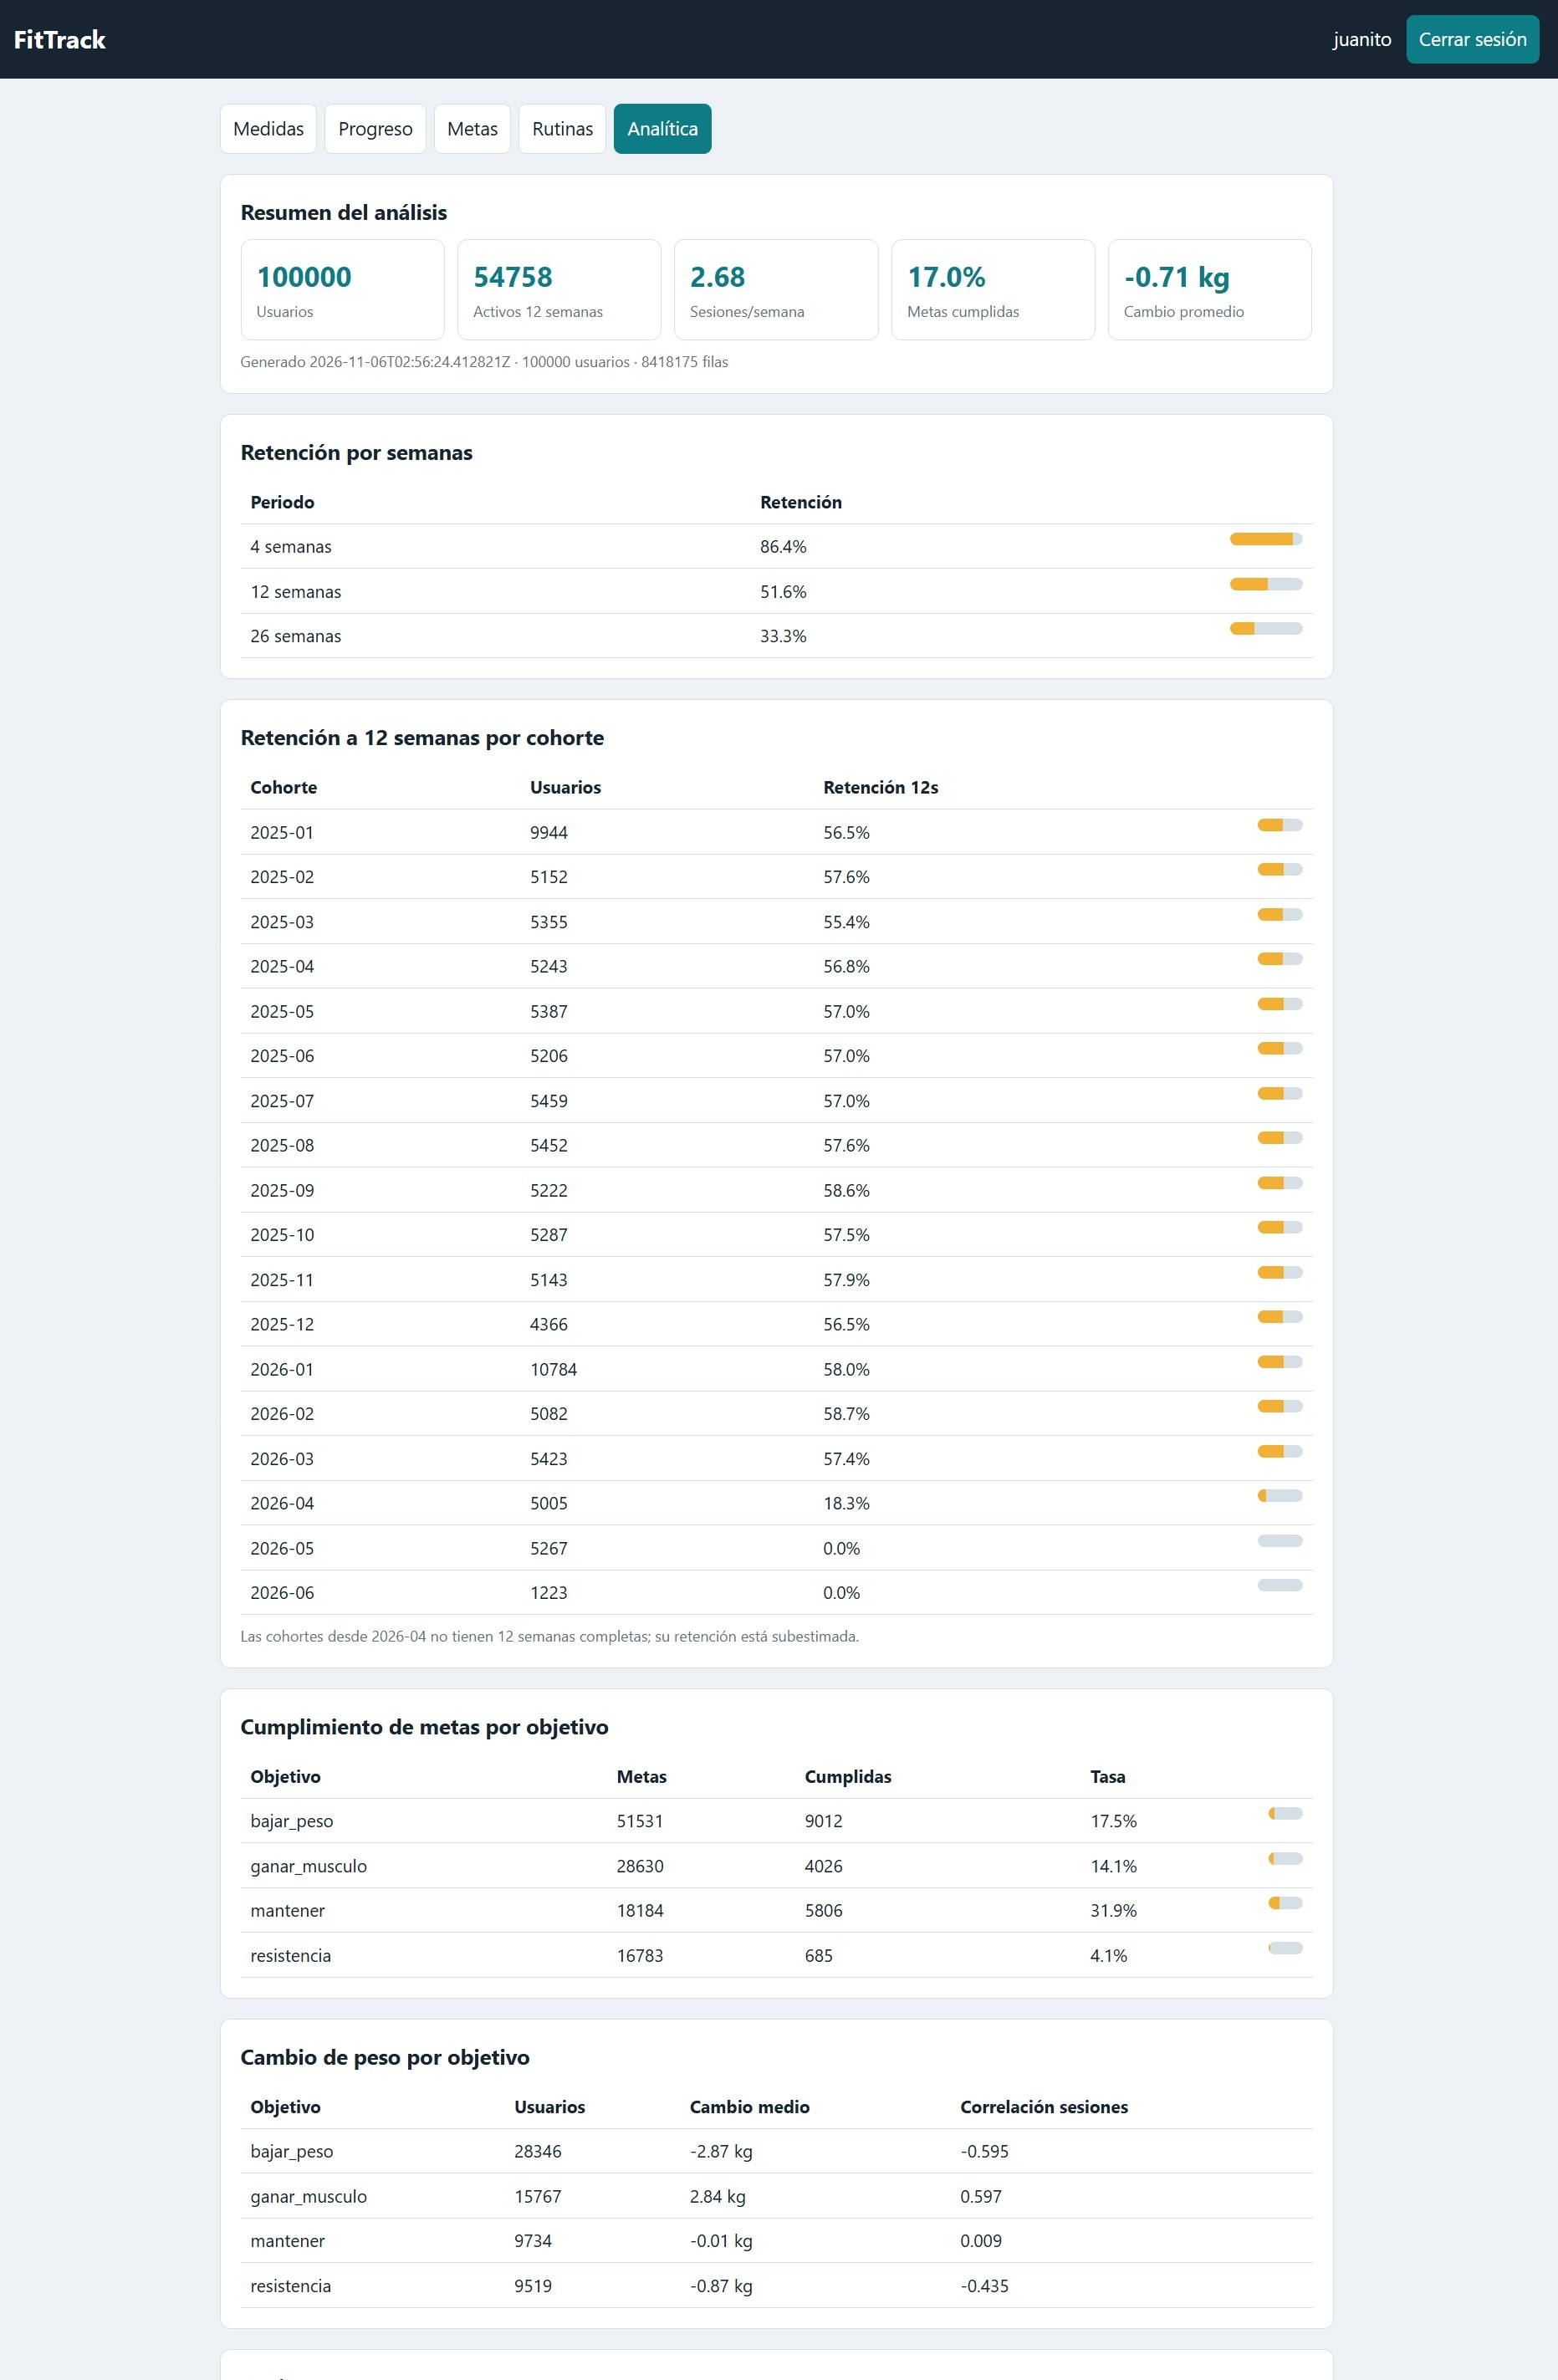
\includegraphics[width=\columnwidth]{figuras/dashboard-crop.jpeg}
\caption{Parte superior de la pestaña ``Analítica'': KPIs, retención y metas.}
\label{fig:dashboard}
\end{figure}

La pestaña muestra 5 tarjetas de KPIs, retención por semanas y por cohorte, metas por objetivo, peso
por objetivo, registros por mes, rutinas por tipo y una validación con etiquetas verdes
(Figura~\ref{fig:dashboard}). La captura completa está en \texttt{report/figuras/dashboard.jpeg}.

\subsection{Discusión}
\textbf{Fortalezas}: solución completa, reproducible y con evidencia; separación clara entre app y
analítica; validación contra patrones conocidos; documentación de problemas y decisiones.
\textbf{Limitaciones}: dataset sintético; un solo worker de Spark; las bases son instancias únicas;
el failover probado es de tarea, no de nodo ni de base; los KPIs son batch, no tiempo real; la
distribución multi-nodo está probada, pero el throughput no mejora por la red overlay y el worker de
2 cores; el servidor compite con el stack.
\textbf{Riesgos}: memoria y
swap al correr Spark con el stack; tareas huérfanas de intentos anteriores; la rama \texttt{main}
del repo no refleja la versión Docker.

\section{Conclusiones y trabajo futuro}
Se desplegó FitTrack en Docker Swarm con balanceo, se construyó un pipeline de Spark para 8,4 M de
filas y se publicaron los resultados en el dashboard. Las pruebas funcionales, de carga, de
distribución multi-nodo, de estrés y de failover confirman que la solución cumple los objetivos. El
escalado a tres réplicas en un nodo casi duplicó el throughput (72,05 RPS, 0 errores); la
distribución entre los dos nodos se demostró con 2+1 y 1+2 réplicas, aunque el rendimiento bajó a
53--54 RPS por la red overlay y el worker de 2 cores. El estrés marcó una meseta de $\approx$60 RPS y
timeouts desde 100 conexiones. En el failover, matar una de tres tareas dejó el servicio en
99,70\,\% de éxito, con el p95 intacto y recuperación en 8 segundos.

Trabajo futuro: (1) Spark de dos nodos con un filesystem compartido (NFS) o HDFS para que el Parquet
no quede repartido entre nodos y medir 1 vs 2 workers; (2) replicar las bases de datos
(Postgres/MySQL/Mongo) para eliminar el punto único de fallo; (3) \texttt{option redispatch} y
\texttt{retries} en HAProxy para que el cliente no reciba los \texttt{502} del hueco entre la muerte
de la tarea y la retirada de su IP del DNS; (4) streaming con Structured Streaming \cite{streaming}
para KPIs en tiempo real; (5) observabilidad con Prometheus/Grafana y alertas; (6) CI/CD para
construir y publicar imágenes automáticamente; y (7) datos reales anonimizados, si el profesor lo
permite, para contrastar los hallazgos.

\begin{thebibliography}{8}
\bibitem{docker} Docker Inc., \emph{Docker Swarm mode overview}.
\url{https://docs.docker.com/engine/swarm/}
\bibitem{spark} Apache Software Foundation, \emph{Spark SQL, DataFrames and Datasets Guide}.
\url{https://spark.apache.org/docs/latest/sql-programming-guide.html}
\bibitem{ieee} IEEE, \emph{IEEE Conference Template}.
\url{https://www.ieee.org/conferences/publishing/templates.html}
\bibitem{dataset} FitTrack-Synth, generador y validador del dataset, carpeta \texttt{dataset/}.
\bibitem{haproxy} HAProxy Technologies, \emph{HAProxy Configuration Manual}.
\url{https://docs.haproxy.org/}
\bibitem{fastapi} FastAPI, \emph{FastAPI documentation}. \url{https://fastapi.tiangolo.com/}
\bibitem{fittrack} FitTrack, repositorio del proyecto, rama \texttt{proyecto-final}, tag
\texttt{v3.8-proyecto-final}. \url{https://github.com/nicocpxmd/fittrack}
\bibitem{streaming} Apache Software Foundation, \emph{Structured Streaming Programming Guide}.
\url{https://spark.apache.org/docs/latest/structured-streaming-programming-guide.html}
\end{thebibliography}

\end{document}
